\chapter{Filter Graph Editor}
\label{grapheditor}

\section{Introduction}

The filter graph editor allows complex signal processing pipelines to be developed in a graphical fashion. It may be
accessed from the \menustyle{Window | Filter Graph} menu item.

The graph editor view (Fig. \ref{graph-editor}) shows nodes for every instrument channel, trigger, and filter block in
the current session. As new instruments, channels, and filter blocks are added to the session, new nodes will
automatically appear in the graph editor view. Nodes cannot overlap and will automatically move out of the way if
another node is dragged on top of them.

\begin{figure}[H]
\centering
\bigimage{ng-images/graph-editor.png}
\caption{Filter graph editor showing instrument channels and several processing blocks}
\label{graph-editor}
\end{figure}

\section{Interaction}

The view may be zoomed with the mouse wheel, or panned by dragging with the right mouse button, to navigate large
filter graphs which do not fit on a single screen at a reasonable zoom level. Right clicking on a node opens a pop-up
properties view (Fig. \ref{graph-editor-properties}).

\begin{figure}[H]
\centering
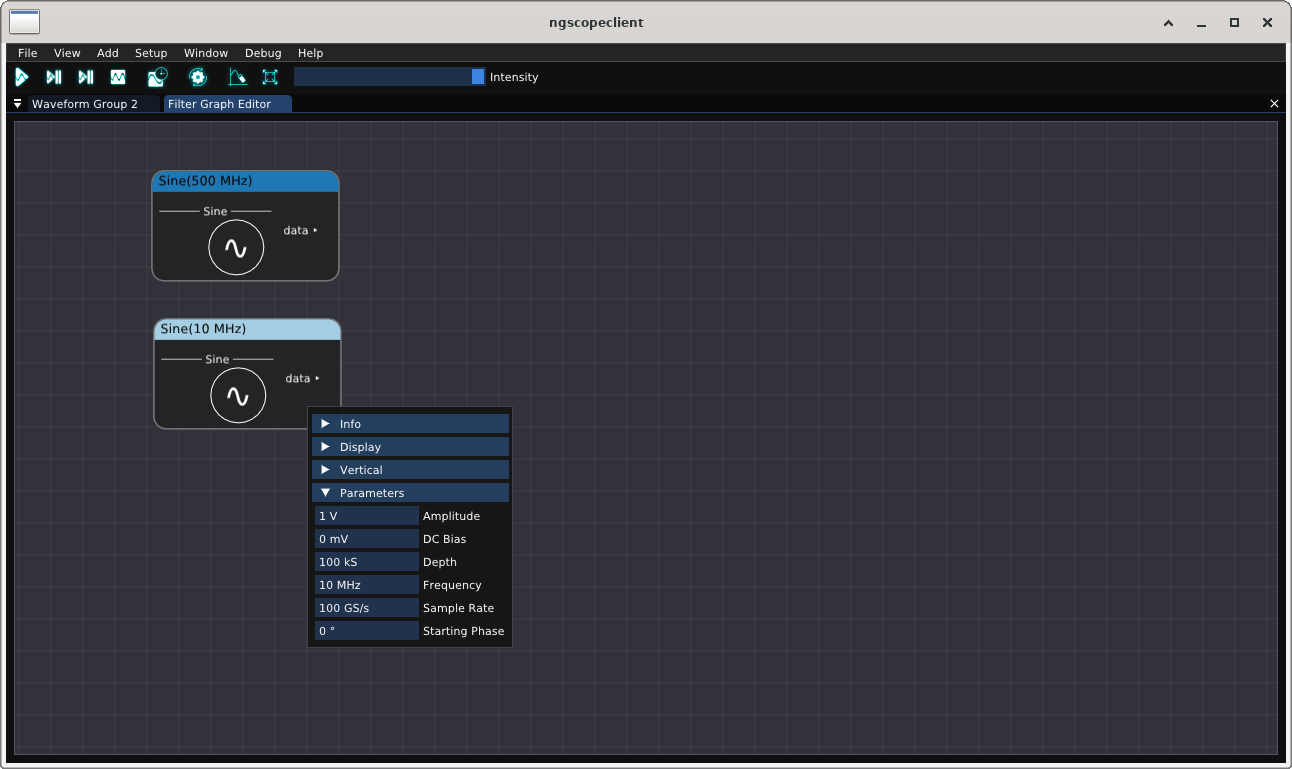
\includegraphics[width=8cm]{ng-images/graph-editor-properties.png}
\caption{Filter graph editor showing properties popup}
\label{graph-editor-properties}
\end{figure}

Nodes display inputs at left and outputs at right. To connect two existing nodes, click on an input or output port and
drag to the port you wish to connect it to. An input can only connect to one output at a time; if the destination
already is connected to a different signal the previous connection will be removed and replaced with the new one.

A tooltip with a green plus sign is displayed during dragging if the proposed connection is valid. If the tooltip
displays a red X instead, the connection is invalid (connecting two inputs, two outputs, or an input and output of
incompatible data types).

To create a new node, click on an input or output port and drag to an empty area of the canvas (Fig.
\ref{graph-editor-create}, Fig. \ref{graph-editor-addinput}). A context menu will appear, presenting a list of filters
which can accept (if dragging from an output) or produce (if dragging from an input) the desired data type. If dragging
from an input, the context menu will also include any currently unused instrument channels.

\begin{figure}[H]
\centering
\bigimage{ng-images/graph-editor-create.png}
\caption{Filter graph editor dragging from an output to an empty area of the canvas}
\label{graph-editor-create}
\end{figure}

\begin{figure}[H]
\centering
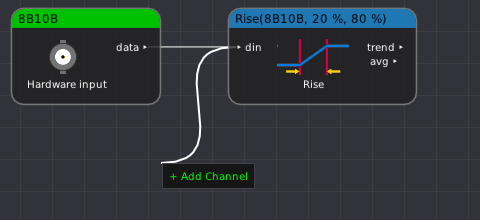
\includegraphics[width=10cm]{ng-images/graph-editor-addinput.png}
\caption{Filter graph editor dragging from an input to an empty area of the canvas}
\label{graph-editor-addinput}
\end{figure}

When a new node is added to the filter graph, each output channel will be automatically added to an existing waveform
view if a compatible one is present. If no compatible view is available, a new view and/or group will be created.

Node title bars are color-coded to match the display color of the waveform trace, allowing easy navigation between
waveform views and the graph editor.

Each node also includes a caption stating the type of node (``hardware input", ``hardware output", or the name of the
filter block) and, in most cases, an icon depicting the functionality of the block.\footnote{Not all filters currently
have icons. We are working with multiple artists to create more filter icons and welcome additional contributions.}

\section{Grouping}

In order to better organize complex experimental setups, nodes may be organized in groups. Groups cannot be nested.

To create a group, right click an unused area of the graph editor canvas and select ``New Group" from the context menu.
This will spawn a new, empty group near the mouse cursor position.

The group will have an automatically generated name (Fig. \ref{graph-editor-group1}) by default. This name may be
changed by right clicking on the group's title bar and typing a new name in the pop-up.

\begin{figure}[H]
\centering
\bigimage{ng-images/graph-editor-group1.png}
\caption{Newly created node group}
\label{graph-editor-group1}
\end{figure}

To add a node to a group, simply drag the node by its title bar and move it into the group (Fig.
\ref{graph-editor-group2}). All paths from the node to the remainder of the filter graph will be routed through
``hierarchical ports" at the left and right edges of the group, reducing clutter. Nodes may be freely moved around
within the group to organize them, or dragged out of the group to remove them from the group.

A group (together with its contents) may be moved by dragging the group's title bar with the left mouse button, or
resized by dragging any of its corners. When a group is moved, it will push other nodes or groups out of the way to
prevent overlapping.

If not needed, a group can be deleted by selecting it with the left mouse button and pressing the ``delete" key.
Deleting a group does not remove any nodes contained within it.

\begin{figure}[H]
\centering
\bigimage{ng-images/graph-editor-group2.png}
\caption{Groups containing several nodes with hierarchical ports}
\label{graph-editor-group2}
\end{figure}
